\documentclass{article}
\iffalse
This file is protected by Copyright. Please refer to the COPYRIGHT file
distributed with this source distribution.

This file is part of OpenCPI <http://www.opencpi.org>

OpenCPI is free software: you can redistribute it and/or modify it under the
terms of the GNU Lesser General Public License as published by the Free Software
Foundation, either version 3 of the License, or (at your option) any later
version.

OpenCPI is distributed in the hope that it will be useful, but WITHOUT ANY
WARRANTY; without even the implied warranty of MERCHANTABILITY or FITNESS FOR A
PARTICULAR PURPOSE. See the GNU Lesser General Public License for more details.

You should have received a copy of the GNU Lesser General Public License along
with this program. If not, see <http://www.gnu.org/licenses/>.
\fi

% TODO: Version numbers?
\usepackage{graphicx}
\graphicspath{ {figures/} }
\usepackage{fancyhdr}
\usepackage{colortbl}
\usepackage[margin=.75in]{geometry}
\usepackage[justification=centering]{caption}
\pagestyle{fancy}
\lhead{Zipper/Myriad-RF 1 Daughtercards}
\rhead{ANGRYVIPER Team}
\definecolor{drkgreen}{rgb}{0,.6,0}
\renewcommand{\headrulewidth}{0pt}
\definecolor{blue}{rgb}{.7,.8,.9}
\begin{document}
\section*{zipper\_i2c.test}
To support the zipper\_i2c.test application on the Zedboard (zed), Xilinx Virtex6 (ml605), and Altera Stratix 4 (alst4) development kits, 2 daughtercards are required:\par
	\begin{itemize}
	\item[1)] Myriad-RF 1 board
	\item[2)] Zipper FMC/HSMC carrier card for Myriad-RF 1
	\end{itemize}
	\begin{figure}[ht]
	\centering
		\begin{minipage}{.5\textwidth}
			\centering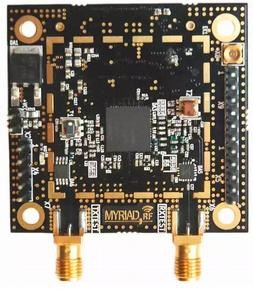
\includegraphics[width=0.65\linewidth]{myriadrf}
			\captionof{figure}{Myriad-RF 1 Board}
			\label{fig:myriadrf}
		\end{minipage}%
		\begin{minipage}{.5\textwidth}
			\centering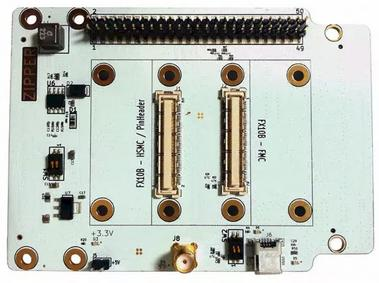
\includegraphics[width=1.0\linewidth]{zipper}
			\captionof{figure}{Zipper FMC/HSMC carrier card for Myriad-RF 1}
			\label{fig:zipper}
		\end{minipage}
	\end{figure}
\noindent Note that the Zipper carrier card requires the hardware modifications specified in \cite{zipper_mods}.

\pagebreak
  \begin{thebibliography}{1}

  \bibitem{zipper_mods} Required Modifications for Myriad-RF 1 and Zipper Daughtercards\\
	 Required\_Modifications\_for\_Myriad-RF\_1\_Zipper\_Daughtercards.pdf (included in cards doc directory)

  \end{thebibliography}
\end{document}
